% Versão 24/06/2020

% Este documento destina-se a servir como modelo para a produção de documentos
% de pesquisa do PPGINF/UFPR, como projetos, dissertações e teses. A classe de
% documento se chama "ppginf" (arquivo ppginf.cls) e define o formato básico do
% documento. O texto está organizado em capítulos que são colocados em
% subdiretórios separados. São definidos exemplos para a inclusão de figuras,
% códigos-fonte e a definição de tabelas.
%
% Produzido por Carlos Maziero (maziero@inf.ufpr.br).

%=====================================================

% Opções da classe ppginf:
%
% - defesa    : versão para entregar à banca; tem espaçamento 1,5
%               e omite algumas páginas iniciais (agradecimentos, etc)
% - final     : versão pós-defesa, para enviar à biblioteca;
%               tem espaçamento simples e todas as páginas iniciais.
% - oneside   : somente frente; use quando for gerar somente o PDF.
% - twoside   : frente/verso; use se precisar de uma versão impressa.
% - metadados : inclui metadados no PDF (por default não inclui)
% - ...       : demais opções aceitas pela classe "book"

% ATENÇÂO: este modelo tem suporte para português e inglês.
% As duas línguas devem ser informadas como opção da classe;
% a língua principal do documento deve vir POR ÚLTIMO.

% Versão de defesa em português
%\documentclass[defesa,oneside,english,brazilian]{ppginf}

% Versão de defesa em inglês
%\documentclass[defesa,oneside,brazilian,english]{ppginf}

% Versão final em PDF para a biblioteca da UFPR (português e inglês)
\documentclass[final,oneside,english,brazilian]{ppginf}
%\documentclass[final,oneside,brazilian,english]{ppginf}

% Versão final para impressão (frente/verso)
%\documentclass[final,twoside,english,brazilian]{ppginf}

% configurações de diversos pacotes, inclusive a fonte usada no texto
% Pacotes usados neste documento e suas respectivas configurações

% ------------------------------------------------------------------------------

% Definição de fontes

% formato dos arquivos-fonte (utf8 no Linux e latin1 no Windows)
\usepackage[utf8]{inputenc}	% arquivos LaTeX em Unicode (UTF8)

% usar codificação T1 para ter caracteres acentuados corretos no PDF
\usepackage[T1]{fontenc}

% fonte usada no corpo do texto (pode alterar, mas descomente apenas uma)
\usepackage{newtxtext,newtxmath}	% Times (se não tiver, use mathptmx)
%\usepackage{lmodern}			% Computer Modern (fonte clássico LaTeX)
%\usepackage{kpfonts}			% Kepler/Palatino (idem, use mathpazo)
%\renewcommand{\familydefault}{\sfdefault} % Arial/Helvética (leia abaixo)

% A biblioteca central da UFPR recomenda usar Arial, seguindo a recomendação da
% ABNT. Essa é uma escolha ruim, pois fontes sans-serif são geralmente inade-
% quados para textos longos e impressos, sendo melhores para páginas Web.
% http://www.webdesignerdepot.com/2013/03/serif-vs-sans-the-final-battle/.

% fontes usadas em ambientes específicos
\usepackage[scaled=0.9]{helvet}		% Sans Serif
\usepackage{courier}			% Verbatim, Listings, etc

% ------------------------------------------------------------------------------

% inclusão de figuras em PDF, PNG, PS, EPS
\usepackage{graphicx}

% subfiguras (subfigure is deprecated, don't use it)
\usepackage[labelformat=simple]{subcaption}
\renewcommand\thesubfigure{(\alph{subfigure})}

% ------------------------------------------------------------------------------

% inclusão/formatação de código-fonte (programas)
\usepackage{listings}
\lstset{language=c}
\lstset{basicstyle=\ttfamily\footnotesize,commentstyle=\textit,stringstyle=\ttfamily}
\lstset{showspaces=false,showtabs=false,showstringspaces=false}
\lstset{numbers=left,stepnumber=1,numberstyle=\tiny}
\lstset{columns=flexible,mathescape=true}
\lstset{frame=single}
\lstset{inputencoding=utf8,extendedchars=true}
\lstset{literate={á}{{\'a}}1  {ã}{{\~a}}1 {à}{{\`a}}1 {â}{{\^a}}1
                 {Á}{{\'A}}1  {Ã}{{\~A}}1 {À}{{\`A}}1 {Â}{{\^A}}1
                 {é}{{\'e}}1  {ê}{{\^e}}1 {É}{{\'E}}1  {Ê}{{\^E}}1
                 {í}{{\'\i}}1 {Í}{{\'I}}1
                 {ó}{{\'o}}1  {õ}{{\~o}}1 {ô}{{\^o}}1
                 {Ó}{{\'O}}1  {Õ}{{\~O}}1 {Ô}{{\^O}}1
                 {ú}{{\'u}}1  {Ú}{{\'U}}1
                 {ç}{{\c{c}}}1 {Ç}{{\c{C}}}1 }

% ------------------------------------------------------------------------------

% formatação de algoritmos
\usepackage{algorithm,algorithmic}
\IfLanguageName{brazilian} {\floatname{algorithm}{Algoritmo}}{}
\renewcommand{\algorithmiccomment}[1]{~~~// #1}
%\algsetup{linenosize=\footnotesize,linenodelimiter=.}

% ------------------------------------------------------------------------------

% formatação de bibliografia
\usepackage{natbib}		% bibliografia no estilo NatBib
\renewcommand{\cite}{\citep}	% \cite deve funcionar como \citep
%\bibpunct{[}{]}{;}{a}{}{,}	% caracteres usados nas referências

% ------------------------------------------------------------------------------

% fontes adicionais
\usepackage{amsmath}		% pacotes matemáticos
\usepackage{amsfonts}		% fontes matemáticas 
\usepackage{amssymb}		% símbolos 

% ------------------------------------------------------------------------------

% pacotes diversos
\usepackage{alltt,moreverb}	% mais comandos no modo verbatim
\usepackage{lipsum}		% gera texto aleatório (para os exemplos)
\usepackage{currfile}		% infos sobre o arquivo/diretório atual
\usepackage[final]{pdfpages}	% inclusão de páginas em PDF
\usepackage{longtable}		% tabelas multi-páginas (tab símbolos/acrônimos)

% ------------------------------------------------------------------------------



%=====================================================

\begin {document}

% Principais dados, usados para gerar as páginas iniciais.
% Campos não utilizados podem ser removidos ou comentados.

% título
\title{Teste Wald para avaliação de parâmetros de regressão e dispersão em modelos multivariados de covariância linear generalizada}

% palavras-chave e keywords (p/ resumo, abstract e metadados do PDF)
\pchave{McGLM. Testes de hipóteses. Teste Wald. ANOVA. MANOVA. Comparações múltiplas. Regressão.}
\keyword{McGLM. Hypothesis tests. Wald test. ANOVA. MANOVA. Multiple comparisons. Regression.}

% autoria
\author{Lineu Alberto Cavazani de Freitas}
\advisor{Prof. Dr. Wagner Hugo Bonat}
\coadvisor{Prof. Dr. Marco Antônio Zanata Alves}

% instituição
\IfLanguageName{brazilian}
  { \instit{UFPR}{Universidade Federal do Paraná} }
% a Bib/UFPR exige que tudo seja em português, exceto o título :-(
%  { \instit{UFPR}{Federal University of Paraná} }
  { \instit{UFPR}{Universidade Federal do Paraná} }

% área de concentração (default do PPGInf, não mudar)
\IfLanguageName{brazilian}
  { \field{Ciência da Computação} }
% a Bib/UFPR exige que tudo seja em português, exceto o título :-(
%  { \field{Computer Science} }
  { \field{Ciência da Computação} }

% data (só o ano)
\date{2022}

% local
\IfLanguageName{brazilian}
  { \local{Curitiba PR} }
% a Bib/UFPR exige que tudo seja em português, exceto o título :-(
%  { \local{Curitiba PR - Brazil} }
  { \local{Curitiba PR} }

% imagem de fundo da capa (se não desejar, basta comentar)
\coverimage{0-iniciais/fundo-capa.jpg}

%=====================================================

%% Descrição do documento (obviamente, descomentar somente UMA!)

% Por exigência da biblioteca da UFPR, a descrição do documento deve ser
% em português, mesmo em documentos em outras línguas. Vá entender...

% tese de doutorado
%\descr{Tese apresentada como requisito parcial à obtenção do grau de Doutor em Ciência da Computação no Programa de Pós-Graduação em Informática, Setor de Ciências Exatas, da Universidade Federal do Paraná}

% exame de qualificação de doutorado
%\descr{Documento apresentado como requisito parcial ao exame de qualificação de Doutorado no Programa de Pós-Graduação em Informática, Setor de Ciências Exatas, da Universidade Federal do Paraná}

% dissertação de mestrado
\descr{Dissertação apresentada como requisito parcial à obtenção do grau de Mestre em Informática no Programa de Pós-Graduação em Informática, Setor de Ciências Exatas, da Universidade Federal do Paraná}

% exame de qualificação de mestrado
%\descr{Documento apresentado como requisito parcial ao exame de qualificação de Mestrado no Programa de Pós-Graduação em Informática, Setor de Ciências Exatas, da Universidade Federal do Paraná}

% trabalho de conclusão de curso
%\descr{Trabalho apresentado como requisito parcial à conclusão do Curso de Bacharelado em XYZ, Setor de Ciências Exatas, da Universidade Federal do Paraná}

% trabalho de disciplina
%\descr{Trabalho apresentado como requisito parcial à conclusão da disciplina XYZ no Curso de Bacharelado em XYZ, Setor de Ciências Exatas, da Universidade Federal do Paraná}

% doctorate thesis
%\descr{Thesis presented as a partial requirement for the degree of Doctor in Computer Science in the Graduate Program in Informatics, Exact Sciences Sector, of the Federal University of Paraná, Brazil}

% doctorate qualification
%\descr{Document presented as a partial requirement for the doctoral qualification exam in the Graduate Program in Informatics, Exact Sciences Sector, of the Federal University of Paraná, Brazil}

% MSc dissertation
%\descr{Dissertation presented as a partial requirement for the degree of Master of Sciences in Informatics in the Graduate Program in Informatics, Exact Sciences Sector, of the Federal University of Paraná, Brazil.}

% MSc qualification
%\descr{Document presented as a partial requirement for the Master of Sciences qualification exam in the Graduate Program in Informatics, Exact Sciences Sector, of the Federal University of Paraná, Brazil}

%=====================================================

% define estilo das páginas iniciais (capas, resumo, sumário, etc)
\frontmatter
\pagestyle{frontmatter}

% produz capa e folha de rosto
\titlepage

% páginas que só aparecem na versão final (a inclusão é automática)
% IMPORTANTE: o conteúdo exato da ficha catalográfica é preparada pela
% Biblioteca da UFPR. Não "invente" um conteúdo para ela!

\begin{ficha}	% só gera conteúdo se for na versão final

% inclusão da ficha catalográfica final (arquivo PDF)
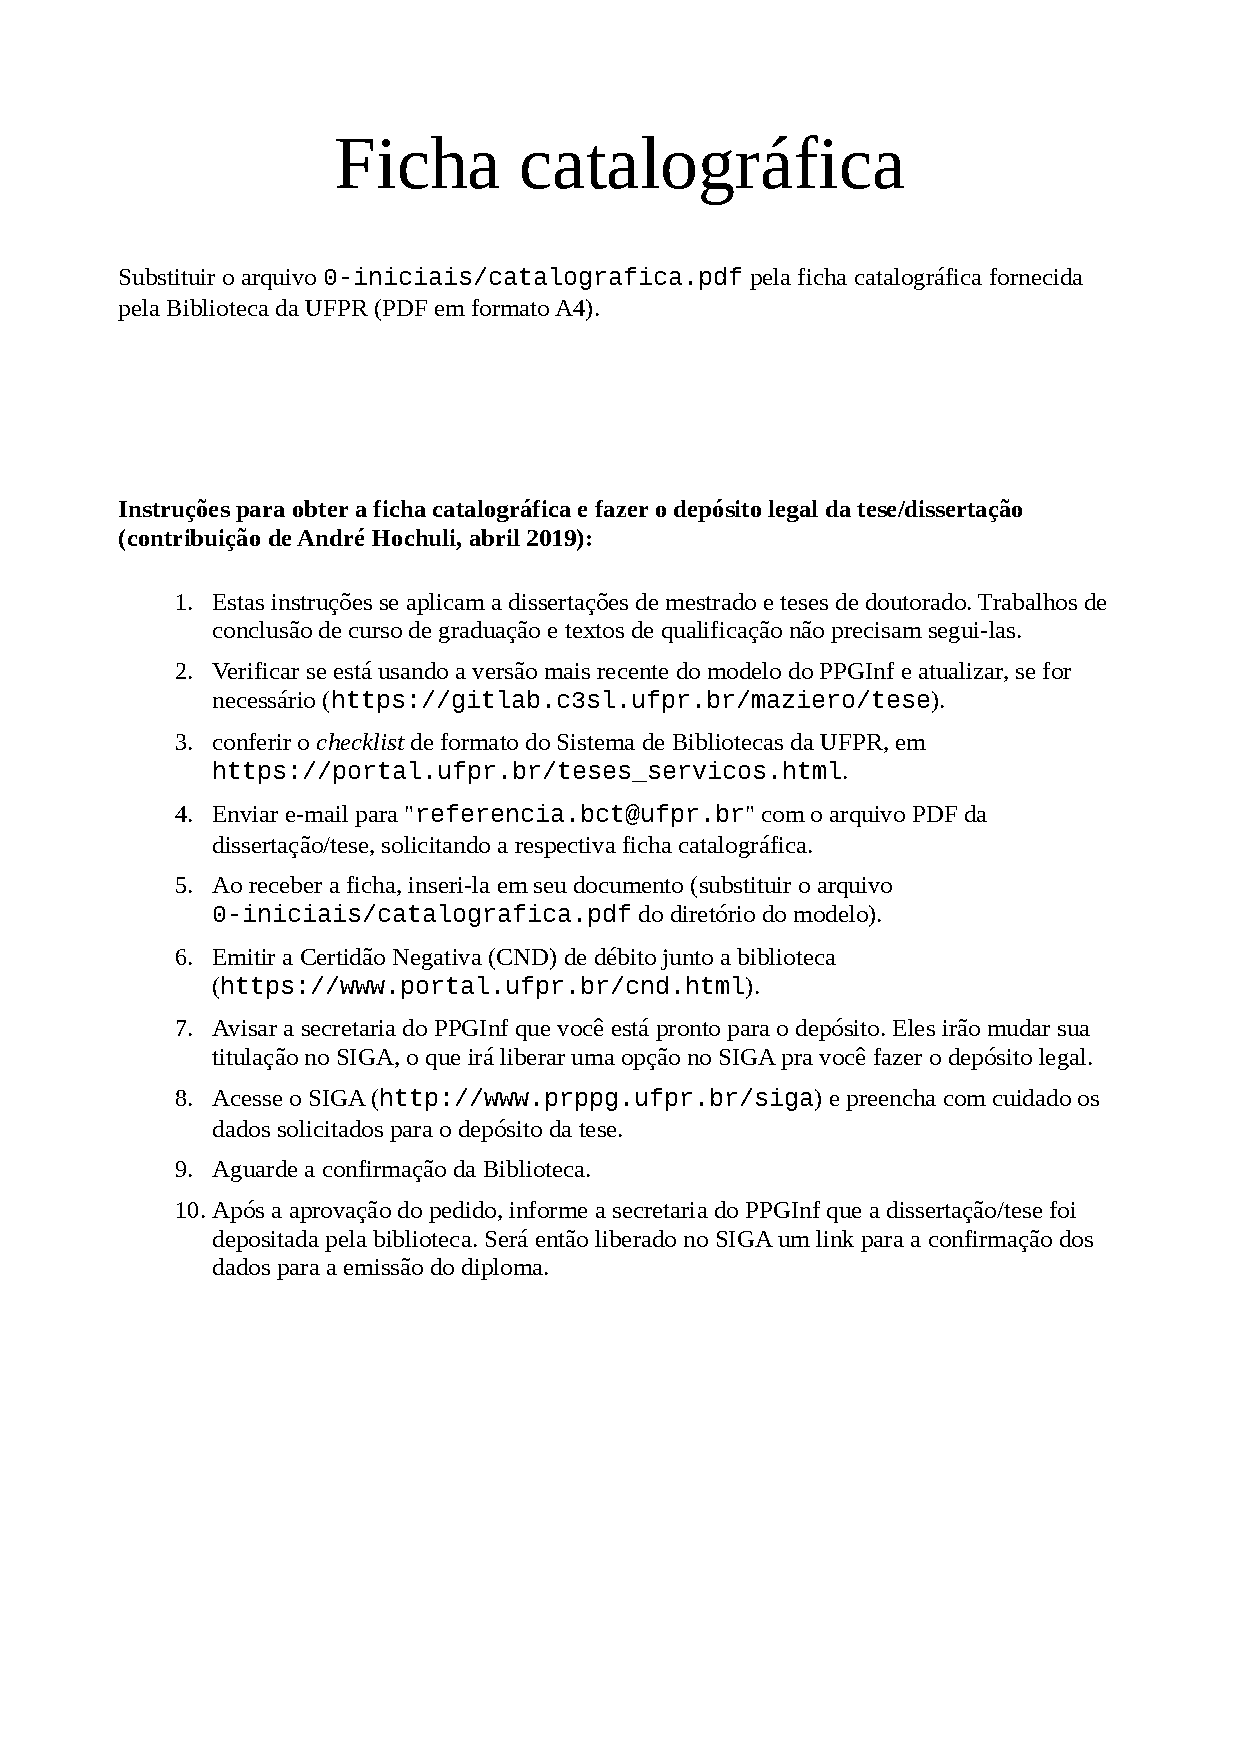
\includepdf[noautoscale]{0-iniciais/catalografica.pdf}

\end{ficha}

%=====================================================
	% ficha catalográfica
% A ficha de aprovação será fornecida pela secretaria do programa,
% após a defesa e cumprimento dos demais trâmites legais.

\begin{aprovacao}	% só gera conteúdo se for na versão final

% inclusão do termo de aprovação final (arquivo PDF)
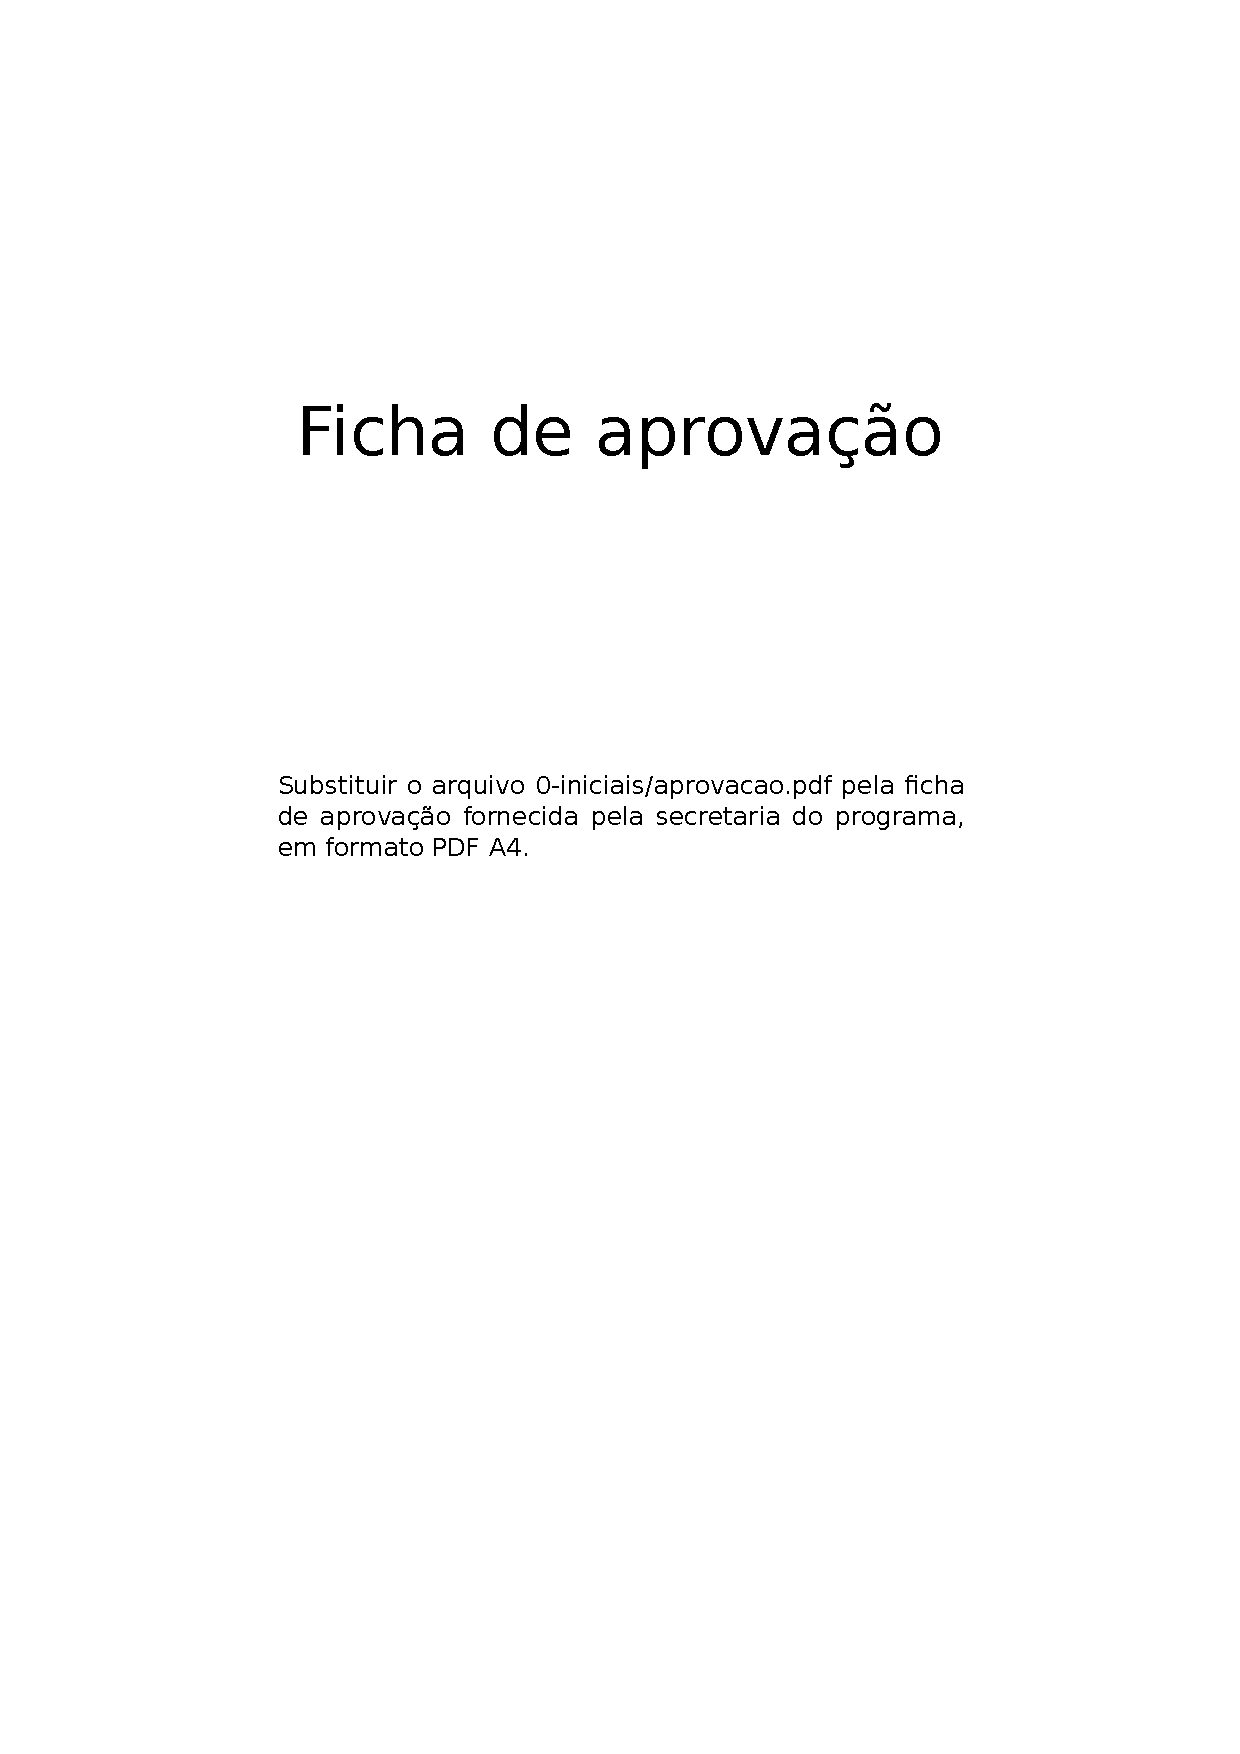
\includepdf[noautoscale]{0-iniciais/aprovacao.pdf}

\end{aprovacao}

%=====================================================
		% folha de aprovação
\begin{dedica}  % só gera conteúdo se for na versão final

"A tentação de formar teorias prematuras sobre dados insuficientes é a ruína da nossa profissão." Sherlock Holmes, de Sir Arthur Conan Doyle

\end{dedica}
		% dedicatória
\begin{agradece}	% só gera conteúdo se for na versão final

À minha família, em especial a meus pais, Hamilton Alves de Freitas e Lúcia Elena Cavazani de Freitas, que mesmo atuando distante de sua realidade nunca deixaram de estar ao meu lado.

Ao meu orientador, Professor Doutor Wagner Hugo Bonat, que me acompanha nesta jornada desde muito antes do ingresso na pós graduação.

Ao professor Professor Doutor Walmes Marques Zeviani, apoiador e conselheiro deste e outros projetos desde a graduação.

Aos professores Wagner e Walmes também agradeço pela confiança depositada em todos os projetos que participei na Ômega - Escola de Data Science.

Aos professores Cesar Augusto Taconeli e José Luiz Padilha da Silva, meus primeiros orientadores em minha trajetória acadêmica e grandes apoiadores da sequência da minha carreira com foco em pesquisa e docência.

Ao professor doutor Paulo Justiniano Ribeiro Junior, pelas experiências ao seu lado na disciplina transversal de métodos estatísticos em pesquisa científica na Universidade Federal do Paraná - MEPC, pelas oportunidades, conversas, risadas e pela maneira gentil que sempre me tratou.

Ao professor doutor Marco Antonio Zanata Alves pelo acolhimento, paciência, por confiar no meu potencial para participar de projetos de linhas de pesquisa que não estou habituado, e pelos valiosos conselhos sobre como tratar do tema desta dissertação para com pessoas com formações diferentes das minhas.

Aos pesquisadores Ligia Oliveira Carlos, Marilia Ramos, Nathalia Wagner, Ingrid Felicidade e Antonio Carlos Campos, do grupo de pesquisa em obesidade, cirurgia bariátrica e microbioma do departamento de clínica cirurgica da Universidade Federal do Paraná, pela disponibilização do conjunto de dados usado para motivar as ideias deste trabalho; em especial à Doutora Ligia Carlos pelo suporte prestado ao longo da elaboração e revisão do trabalho.

A todos os colegas de mestrado, em especial àqueles do grupo de pesquisa HiPES, pelo acolhimento e paciência com um novo colega de formação diferente.

Aos professores dos departamentos de Estatística, Informática e Matemática que fizeram parte da minha trajetória na Universidade Federal do Paraná. Em especial àqueles do Laboratório de Estatística e Geoinformação. 

À Universidade Federal do Paraná - UFPR e ao Programa de Pós Graduação em Informática - PPGINF, incluindo professores e equipe administrativa, pelo brilhante trabalho e resiliência apresentados mesmo em tempos de pandemia.

À Coordenação de Aperfeiçoamento Pessoal de Ensino Superior - CAPES, pelo suporte financeiro nestes anos de pesquisa.

Aos membros da banca de qualificação e defesa da dissertação pelas valiosas contribuições.

À todos que estiveram ao meu lado no decorrer destes anos e contribuíram direta ou indiretamente neste trabalho. 

À todos vocês, meu sincero agradecimento.

\end{agradece}
		% agradecimentos

% resumo (português) e abstract (inglês)
\begin{resumo}

Ciência de dados é um campo de estudo interdisciplinar que compreende áreas como estatística, ciência da computação e matemática. Neste contexto, métodos estatísticos são de fundamental importância sendo que, dentre as possíveis técnicas disponíveis para análise de dados, os modelos de regressão têm papel importante. Tais modelos são indicados a problemas nos quais existe interesse em verificar a associação entre uma ou mais variáveis respostas e um conjunto de variáveis explicativas. Isto é feito através da obtenção de uma equação que explique a relação entre as variáveis explicativas e a(s) resposta(s). Existem modelos uni e multivariados: nos modelos univariados há apenas uma variável resposta; já em modelos multivariados há mais de uma resposta. Dentre as classes de modelos multivariados estão os modelos multivariados de covariância linear generalizada (McGLMs). No contexto de modelos de regressão, é comum o interesse em avaliar os valores dos parâmetros por meio de testes de hipóteses e existem técnicas baseadas em tais testes, como as análises de variâncias univariadas, multivariadas e ainda os testes de comparações múltiplas. No entanto, considerando os McGLMs, não há discussão a respeito do uso destes testes para a classe. Nossa proposta é utilizar o teste Wald para a realização de testes de hipóteses gerais sobre parâmetros de regressão e dispersão de McGLMs. Por meio da avaliação dos parâmetros de regressão é possível identificar qual(is) variável(is) explicativa(s) apresentam efeito sobre a(s) resposta(s). Por meio do estudo dos parâmetros de dispersão pode-se avaliar o efeito da correlação entre unidades do estudo, como por exemplo em estudos longitudinais, temporais e de medidas repetidas. Apresentamos implementações em R de funções para efetuar tais testes, bem como funções para efetuar ANOVAs, MANOVAs e testes de comparações múltiplas. As propriedades e comportamento dos testes propostos foram verificados com base em estudos de simulação e o potencial de aplicação das metodologias discutidas foi motivado com base na aplicação a um conjunto de dados real. Os resultados mostraram que quanto mais distante a hipótese testada é dos valores verdadeiros dos parâmetros, maior é o percentual de rejeição da hipótese nula. Tal como esperado, os menores percentuais de rejeição foram observados quando a hipótese nula testada correspondia aos reais valores dos parâmetros. Também verificou-se que conforme aumenta-se o tamanho amostral, o percentual de rejeição aumenta para hipóteses nulas pouco diferentes dos valores simulados dos parâmetros. Logo, os resultados apontam que o teste Wald pode ser usado para avaliar hipóteses sobre parâmetros de regressão e dispersão de McGLMs, o que permite uma melhor interpretação do efeito das variáveis e estruturas de delineamento em contextos práticos.

\end{resumo}

\begin{abstract}

Data science is an interdisciplinary field of study that comprises areas such as statistics, computer science and mathematics. In this context, statistical methods are of fundamental importance and, among the possible techniques available for data analysis, regression models play an important role. Such models are suitable for problems in which there is an interest in verifying the association between one or more response variables and a set of explanatory variables. This is done by obtaining an equation that explains the relationship between the explanatory variables and the response(s). There are univariate and multivariate models: in univariate models there is only one response variable; in multivariate models there is more than one response. Among the classes of multivariate models are the multivariate covariance generalized linear models (McGLMs). In the context of regression models, there is a common interest in evaluating parameter values through hypothesis tests and there are techniques based on such tests, such as univariate and multivariate analysis of variance and even multiple comparison tests. However, considering the McGLMs, there is no discussion regarding the use of these tests for the class. Our proposal is to use the Wald test to carry out tests of general hypotheses on regression and dispersion parameters of McGLMs. By evaluating the regression parameters, it is possible to identify which explanatory variable(s) have an effect on the response(s). Through the study of dispersion parameters, the effect of the correlation between study units can be evaluated, for example in longitudinal, temporal, and repeated measures studies. We present R implementations of functions to perform such tests, as well as functions to perform ANOVAs, MANOVAs and multiple comparison tests. The properties and behavior of the proposed tests were verified based on simulation studies and the potential of application of the discussed methodologies was motivated based on the application to a real dataset. The results showed that the further the tested hypothesis is from the true values of the parameters, the greater the percentage of rejection of the null hypothesis. As expected, the lowest rejection percentages were observed when the null hypothesis tested corresponded to the real values of the parameters. It was also verified that as the sample size increases, the rejection percentage increases for null hypotheses that are little different from the simulated values of the parameters. Therefore, the results indicate that the Wald test can be used to evaluate hypotheses about regression and dispersion parameters of McGLMs, which allows a better interpretation of the effect of variables and design structures in practical contexts.

\end{abstract}


% listas  de figuras, tabelas, abreviações/siglas, símbolos
\listoffigures				% figuras
\clearpage
\listoftables				% tabelas
%=====================================================

% lista de acrônimos (siglas e abreviações)

\begin{listaacron}

\begin{longtable}[l]{p{0.2\linewidth}p{0.7\linewidth}}

LM & Modelo linear\\
GLM & Modelo linear generalizado\\
cGLM & Modelo de covariância linear generalizada\\
McGLM & Modelo multivariado de covariância linear generalizada\\
ANOVA & Análise de variância\\
MANOVA & Análise de variância multivariada\\
hGLM & Modelo linear generalizado hierárquico\\
GEE & Equações de Estimação Generalizadas\\
GAMLSS & Modelos aditivos generalizados para locação, escala e forma\\
GLMM & Modelos lineares generalizados mistos\\
MGLMM & Modelos lineares generalizados multivariados mistos\\
MLM & Modelos lineares multivariados\\
MGLM & Modelos lineares generalizados multivariados\\
RYGB & Bypass Gástrico em Y de Roux\\
BES & Escala de compulsão alimentar\\
YFAS & Escala de vício alimentar\\


\end{longtable}

\end{listaacron}

%=====================================================
		% acrônimos, deve ser preenchida à mão
%%=====================================================

% lista de símbolos

\begin{listasimb}

\begin{longtable}[l]{p{0.2\linewidth}p{0.7\linewidth}}
$\alpha$ & alfa, primeira letra do alfabeto grego\\
$\beta$ & beta, segunda letra do alfabeto grego\\
$\gamma$ & gama, terceira letra do alfabeto grego\\
$\omega$ & ômega, última letra do alfabeto grego\\
$\pi$ & pi \\
$\tau$ & Tempo de resposta do sistema\\
$\theta$ & Ângulo de incidência do raio luminoso\\
\end{longtable}

\end{listasimb}

%=====================================================
		% símbolos, idem
\tableofcontents			% sumário

%=====================================================

% define estilo do corpo do documento (capítulos e apêndices)
\mainmatter
\pagestyle{mainmatter}

% inclusao de cada capítulo, alterar a gosto (do professor de Metodologia)
\chapter{Estudo de simulação}

%=====================================================

Com o objetivo de avaliar o poder do teste Wald em testes de hipóteses sobre parâmetros de McGLMs, foram executados estudos de simulação. Nestas simulações avaliamos o comportamento da proposta para três distribuições de probabilidade: Normal, Poisson e Bernoulli. Simulamos cenários univariados e também trivariados com diferentes tamanhos amostrais para verificar as propriedades dos testes sobre parâmetros de regressão, dispersão e potência.

Para simular conjuntos de dados univariados foram usadas bibliotecas padrão do R. Para simular conjuntos de dados com múltiplas respostas seguindo distribuição Normal, foi usada a biblioteca R \emph{mvtnorm} \citep{mvtnorm1}, \citep{mvtnorm2}. Para as outras distribuições foi utilizado o método NORTA \citep{cario1997modeling} implementado na biblioteca R \emph{NORTARA} \citep{nortara}.

\section{Parâmetros de regressão}

Para avaliação de hipóteses sobre parâmetros de regressão foram considerados tamanhos amostrais de 50, 100, 250, 500 e 1000. Foram gerados 500 conjuntos de dados para cada tamanho amostral simulando uma situação com uma variável explicativa categórica de 4 níveis. Para distribuição Normal os parâmetros de regressão usados foram: $\beta_0 = 5$, $\beta_1 = 0$, $\beta_2 = 0$, $\beta_3 = 0$. Para a distribuição Poisson os parâmetros de regressão usados foram: $\beta_0 = 2,3$, $\beta_1 = 0$, $\beta_2 = 0$, $\beta_3 = 0$. E para a distribuição Bernoulli os parâmetros de regressão usados foram: $\beta_0 = 0,5$, $\beta_1 = 0$, $\beta_2 = 0$, $\beta_3 = 0$. Os valores foram escolhidos de tal modo que o coeficiente de variação para distribuição Normal fosse de 20\%, as contagens para Poisson fossem próximas de 10 e a probabilidade de sucesso da Bernoulli fosse aproximadamente 0,6. Foram avaliados cenários univariados e trivariados com estas características. Para os cenários trivariados, existem 4 parâmetros por resposta que seguem as configurações descritas.

Para cada amostra gerada foi ajustado um McGLM em que, para os conjuntos com variáveis respostas seguindo distribuição Normal a função de ligação utilizada foi a identidade com função de variância constante. Para Poisson a função de ligação utilizada foi a logarítmica e para função de variância utilizou-se a Tweedie. Já para as respostas seguindo distribuição Bernoulli foi utilizada a função de ligação logito com função de variância Binomial. Em todos os casos o preditor matricial para a matriz de
variância e covariância foi especificado de forma a explicitar que as observações são independentes dentro de cada resposta. A correlação entre respostas no caso trivariado é dada pela matriz $\Sigma_b$:

$$
\Sigma_b = 
\begin{bmatrix}
1    & 0,75 & 0,5  \\
0,75 & 1    & 0,25 \\
0,5  & 0,25 & 1    \\
\end{bmatrix}
$$

Com os modelos ajustados, o procedimento consistiu em variar as hipóteses testadas sobre os parâmetros simulados. Consideramos 20 diferentes hipóteses baseadas em um decréscimo de $\beta_0/20$ e distribuição deste decréscimo nos demais $\beta$s da hipótese nula. Para cada ponto avaliamos o percentual de rejeição da hipótese nula. A ideia é verificar o que ocorre quando afastamos as hipóteses nulas dos reais valores dos parâmetros. Espera-se que no primeiro ponto haja um percentual de rejeição baixo, pois a hipótese nula corresponde aos reais valores dos parâmetros. Para os demais pontos espera-se que o percentual de rejeição aumente gradativamente, pois as hipóteses afastam-se dos valores originalmente simulados.

Para representar graficamente os resultados tomamos a distância euclideana de cada vetor de hipóteses com relação ao vetor usado para simular os dados. Adicionalmente dividimos o vetor de distâncias pelo desvio padrão das distância para obter distâncias em uma mesma escala, independente dos parâmetros de regressão. Os resultados são apresentados na \autoref{}.

\section{Parâmetros de dispersão}

\section{Parâmetros de potência}

\textbf{TODO}

\begin{itemize}
  
  \item \textbf{ACRESCENTAR GRÁFICOS}
  
  \item \textbf{}
  
\end{itemize}


%=====================================================

\chapter{Estudo de simulação}

%=====================================================

Com o objetivo de avaliar o poder do teste Wald em testes de hipóteses sobre parâmetros de McGLMs, foram executados estudos de simulação. Nestas simulações avaliamos o comportamento da proposta para três distribuições de probabilidade: Normal, Poisson e Bernoulli. Simulamos cenários univariados e também trivariados com diferentes tamanhos amostrais para verificar as propriedades dos testes sobre parâmetros de regressão, dispersão e potência.

Para simular conjuntos de dados univariados foram usadas bibliotecas padrão do R. Para simular conjuntos de dados com múltiplas respostas seguindo distribuição Normal, foi usada a biblioteca R \emph{mvtnorm} \citep{mvtnorm1}, \citep{mvtnorm2}. Para as outras distribuições foi utilizado o método NORTA \citep{cario1997modeling} implementado na biblioteca R \emph{NORTARA} \citep{nortara}.

\section{Parâmetros de regressão}

Para avaliação de hipóteses sobre parâmetros de regressão foram considerados tamanhos amostrais de 50, 100, 250, 500 e 1000. Foram gerados 500 conjuntos de dados para cada tamanho amostral simulando uma situação com uma variável explicativa categórica de 4 níveis. Para distribuição Normal os parâmetros de regressão usados foram: $\beta_0 = 5$, $\beta_1 = 0$, $\beta_2 = 0$, $\beta_3 = 0$. Para a distribuição Poisson os parâmetros de regressão usados foram: $\beta_0 = 2,3$, $\beta_1 = 0$, $\beta_2 = 0$, $\beta_3 = 0$. E para a distribuição Bernoulli os parâmetros de regressão usados foram: $\beta_0 = 0,5$, $\beta_1 = 0$, $\beta_2 = 0$, $\beta_3 = 0$. Os valores foram escolhidos de tal modo que o coeficiente de variação para distribuição Normal fosse de 20\%, as contagens para Poisson fossem próximas de 10 e a probabilidade de sucesso da Bernoulli fosse aproximadamente 0,6. Foram avaliados cenários univariados e trivariados com estas características. Para os cenários trivariados, existem 4 parâmetros por resposta que seguem as configurações descritas.

Para cada amostra gerada foi ajustado um McGLM em que, para os conjuntos com variáveis respostas seguindo distribuição Normal a função de ligação utilizada foi a identidade com função de variância constante. Para Poisson a função de ligação utilizada foi a logarítmica e para função de variância utilizou-se a Tweedie. Já para as respostas seguindo distribuição Bernoulli foi utilizada a função de ligação logito com função de variância Binomial. Em todos os casos o preditor matricial para a matriz de
variância e covariância foi especificado de forma a explicitar que as observações são independentes dentro de cada resposta. A correlação entre respostas no caso trivariado é dada pela matriz $\Sigma_b$:

$$
\Sigma_b = 
\begin{bmatrix}
1    & 0,75 & 0,5  \\
0,75 & 1    & 0,25 \\
0,5  & 0,25 & 1    \\
\end{bmatrix}
$$

Com os modelos ajustados, o procedimento consistiu em variar as hipóteses testadas sobre os parâmetros simulados. Consideramos 20 diferentes hipóteses baseadas em um decréscimo de $\beta_0/20$ e distribuição deste decréscimo nos demais $\beta$s da hipótese nula. Para cada ponto avaliamos o percentual de rejeição da hipótese nula. A ideia é verificar o que ocorre quando afastamos as hipóteses nulas dos reais valores dos parâmetros. Espera-se que no primeiro ponto haja um percentual de rejeição baixo, pois a hipótese nula corresponde aos reais valores dos parâmetros. Para os demais pontos espera-se que o percentual de rejeição aumente gradativamente, pois as hipóteses afastam-se dos valores originalmente simulados.

Para representar graficamente os resultados tomamos a distância euclideana de cada vetor de hipóteses com relação ao vetor usado para simular os dados. Adicionalmente dividimos o vetor de distâncias pelo desvio padrão das distância para obter distâncias em uma mesma escala, independente dos parâmetros de regressão. Os resultados são apresentados na \autoref{}.

\section{Parâmetros de dispersão}

\section{Parâmetros de potência}

\textbf{TODO}

\begin{itemize}
  
  \item \textbf{ACRESCENTAR GRÁFICOS}
  
  \item \textbf{}
  
\end{itemize}


%=====================================================

\chapter{Estudo de simulação}

%=====================================================

Com o objetivo de avaliar o poder do teste Wald em testes de hipóteses sobre parâmetros de McGLMs, foram executados estudos de simulação. Nestas simulações avaliamos o comportamento da proposta para três distribuições de probabilidade: Normal, Poisson e Bernoulli. Simulamos cenários univariados e também trivariados com diferentes tamanhos amostrais para verificar as propriedades dos testes sobre parâmetros de regressão, dispersão e potência.

Para simular conjuntos de dados univariados foram usadas bibliotecas padrão do R. Para simular conjuntos de dados com múltiplas respostas seguindo distribuição Normal, foi usada a biblioteca R \emph{mvtnorm} \citep{mvtnorm1}, \citep{mvtnorm2}. Para as outras distribuições foi utilizado o método NORTA \citep{cario1997modeling} implementado na biblioteca R \emph{NORTARA} \citep{nortara}.

\section{Parâmetros de regressão}

Para avaliação de hipóteses sobre parâmetros de regressão foram considerados tamanhos amostrais de 50, 100, 250, 500 e 1000. Foram gerados 500 conjuntos de dados para cada tamanho amostral simulando uma situação com uma variável explicativa categórica de 4 níveis. Para distribuição Normal os parâmetros de regressão usados foram: $\beta_0 = 5$, $\beta_1 = 0$, $\beta_2 = 0$, $\beta_3 = 0$. Para a distribuição Poisson os parâmetros de regressão usados foram: $\beta_0 = 2,3$, $\beta_1 = 0$, $\beta_2 = 0$, $\beta_3 = 0$. E para a distribuição Bernoulli os parâmetros de regressão usados foram: $\beta_0 = 0,5$, $\beta_1 = 0$, $\beta_2 = 0$, $\beta_3 = 0$. Os valores foram escolhidos de tal modo que o coeficiente de variação para distribuição Normal fosse de 20\%, as contagens para Poisson fossem próximas de 10 e a probabilidade de sucesso da Bernoulli fosse aproximadamente 0,6. Foram avaliados cenários univariados e trivariados com estas características. Para os cenários trivariados, existem 4 parâmetros por resposta que seguem as configurações descritas.

Para cada amostra gerada foi ajustado um McGLM em que, para os conjuntos com variáveis respostas seguindo distribuição Normal a função de ligação utilizada foi a identidade com função de variância constante. Para Poisson a função de ligação utilizada foi a logarítmica e para função de variância utilizou-se a Tweedie. Já para as respostas seguindo distribuição Bernoulli foi utilizada a função de ligação logito com função de variância Binomial. Em todos os casos o preditor matricial para a matriz de
variância e covariância foi especificado de forma a explicitar que as observações são independentes dentro de cada resposta. A correlação entre respostas no caso trivariado é dada pela matriz $\Sigma_b$:

$$
\Sigma_b = 
\begin{bmatrix}
1    & 0,75 & 0,5  \\
0,75 & 1    & 0,25 \\
0,5  & 0,25 & 1    \\
\end{bmatrix}
$$

Com os modelos ajustados, o procedimento consistiu em variar as hipóteses testadas sobre os parâmetros simulados. Consideramos 20 diferentes hipóteses baseadas em um decréscimo de $\beta_0/20$ e distribuição deste decréscimo nos demais $\beta$s da hipótese nula. Para cada ponto avaliamos o percentual de rejeição da hipótese nula. A ideia é verificar o que ocorre quando afastamos as hipóteses nulas dos reais valores dos parâmetros. Espera-se que no primeiro ponto haja um percentual de rejeição baixo, pois a hipótese nula corresponde aos reais valores dos parâmetros. Para os demais pontos espera-se que o percentual de rejeição aumente gradativamente, pois as hipóteses afastam-se dos valores originalmente simulados.

Para representar graficamente os resultados tomamos a distância euclideana de cada vetor de hipóteses com relação ao vetor usado para simular os dados. Adicionalmente dividimos o vetor de distâncias pelo desvio padrão das distância para obter distâncias em uma mesma escala, independente dos parâmetros de regressão. Os resultados são apresentados na \autoref{}.

\section{Parâmetros de dispersão}

\section{Parâmetros de potência}

\textbf{TODO}

\begin{itemize}
  
  \item \textbf{ACRESCENTAR GRÁFICOS}
  
  \item \textbf{}
  
\end{itemize}


%=====================================================

\chapter{Estudo de simulação}

%=====================================================

Com o objetivo de avaliar o poder do teste Wald em testes de hipóteses sobre parâmetros de McGLMs, foram executados estudos de simulação. Nestas simulações avaliamos o comportamento da proposta para três distribuições de probabilidade: Normal, Poisson e Bernoulli. Simulamos cenários univariados e também trivariados com diferentes tamanhos amostrais para verificar as propriedades dos testes sobre parâmetros de regressão, dispersão e potência.

Para simular conjuntos de dados univariados foram usadas bibliotecas padrão do R. Para simular conjuntos de dados com múltiplas respostas seguindo distribuição Normal, foi usada a biblioteca R \emph{mvtnorm} \citep{mvtnorm1}, \citep{mvtnorm2}. Para as outras distribuições foi utilizado o método NORTA \citep{cario1997modeling} implementado na biblioteca R \emph{NORTARA} \citep{nortara}.

\section{Parâmetros de regressão}

Para avaliação de hipóteses sobre parâmetros de regressão foram considerados tamanhos amostrais de 50, 100, 250, 500 e 1000. Foram gerados 500 conjuntos de dados para cada tamanho amostral simulando uma situação com uma variável explicativa categórica de 4 níveis. Para distribuição Normal os parâmetros de regressão usados foram: $\beta_0 = 5$, $\beta_1 = 0$, $\beta_2 = 0$, $\beta_3 = 0$. Para a distribuição Poisson os parâmetros de regressão usados foram: $\beta_0 = 2,3$, $\beta_1 = 0$, $\beta_2 = 0$, $\beta_3 = 0$. E para a distribuição Bernoulli os parâmetros de regressão usados foram: $\beta_0 = 0,5$, $\beta_1 = 0$, $\beta_2 = 0$, $\beta_3 = 0$. Os valores foram escolhidos de tal modo que o coeficiente de variação para distribuição Normal fosse de 20\%, as contagens para Poisson fossem próximas de 10 e a probabilidade de sucesso da Bernoulli fosse aproximadamente 0,6. Foram avaliados cenários univariados e trivariados com estas características. Para os cenários trivariados, existem 4 parâmetros por resposta que seguem as configurações descritas.

Para cada amostra gerada foi ajustado um McGLM em que, para os conjuntos com variáveis respostas seguindo distribuição Normal a função de ligação utilizada foi a identidade com função de variância constante. Para Poisson a função de ligação utilizada foi a logarítmica e para função de variância utilizou-se a Tweedie. Já para as respostas seguindo distribuição Bernoulli foi utilizada a função de ligação logito com função de variância Binomial. Em todos os casos o preditor matricial para a matriz de
variância e covariância foi especificado de forma a explicitar que as observações são independentes dentro de cada resposta. A correlação entre respostas no caso trivariado é dada pela matriz $\Sigma_b$:

$$
\Sigma_b = 
\begin{bmatrix}
1    & 0,75 & 0,5  \\
0,75 & 1    & 0,25 \\
0,5  & 0,25 & 1    \\
\end{bmatrix}
$$

Com os modelos ajustados, o procedimento consistiu em variar as hipóteses testadas sobre os parâmetros simulados. Consideramos 20 diferentes hipóteses baseadas em um decréscimo de $\beta_0/20$ e distribuição deste decréscimo nos demais $\beta$s da hipótese nula. Para cada ponto avaliamos o percentual de rejeição da hipótese nula. A ideia é verificar o que ocorre quando afastamos as hipóteses nulas dos reais valores dos parâmetros. Espera-se que no primeiro ponto haja um percentual de rejeição baixo, pois a hipótese nula corresponde aos reais valores dos parâmetros. Para os demais pontos espera-se que o percentual de rejeição aumente gradativamente, pois as hipóteses afastam-se dos valores originalmente simulados.

Para representar graficamente os resultados tomamos a distância euclideana de cada vetor de hipóteses com relação ao vetor usado para simular os dados. Adicionalmente dividimos o vetor de distâncias pelo desvio padrão das distância para obter distâncias em uma mesma escala, independente dos parâmetros de regressão. Os resultados são apresentados na \autoref{}.

\section{Parâmetros de dispersão}

\section{Parâmetros de potência}

\textbf{TODO}

\begin{itemize}
  
  \item \textbf{ACRESCENTAR GRÁFICOS}
  
  \item \textbf{}
  
\end{itemize}


%=====================================================

\chapter{Estudo de simulação}

%=====================================================

Com o objetivo de avaliar o poder do teste Wald em testes de hipóteses sobre parâmetros de McGLMs, foram executados estudos de simulação. Nestas simulações avaliamos o comportamento da proposta para três distribuições de probabilidade: Normal, Poisson e Bernoulli. Simulamos cenários univariados e também trivariados com diferentes tamanhos amostrais para verificar as propriedades dos testes sobre parâmetros de regressão, dispersão e potência.

Para simular conjuntos de dados univariados foram usadas bibliotecas padrão do R. Para simular conjuntos de dados com múltiplas respostas seguindo distribuição Normal, foi usada a biblioteca R \emph{mvtnorm} \citep{mvtnorm1}, \citep{mvtnorm2}. Para as outras distribuições foi utilizado o método NORTA \citep{cario1997modeling} implementado na biblioteca R \emph{NORTARA} \citep{nortara}.

\section{Parâmetros de regressão}

Para avaliação de hipóteses sobre parâmetros de regressão foram considerados tamanhos amostrais de 50, 100, 250, 500 e 1000. Foram gerados 500 conjuntos de dados para cada tamanho amostral simulando uma situação com uma variável explicativa categórica de 4 níveis. Para distribuição Normal os parâmetros de regressão usados foram: $\beta_0 = 5$, $\beta_1 = 0$, $\beta_2 = 0$, $\beta_3 = 0$. Para a distribuição Poisson os parâmetros de regressão usados foram: $\beta_0 = 2,3$, $\beta_1 = 0$, $\beta_2 = 0$, $\beta_3 = 0$. E para a distribuição Bernoulli os parâmetros de regressão usados foram: $\beta_0 = 0,5$, $\beta_1 = 0$, $\beta_2 = 0$, $\beta_3 = 0$. Os valores foram escolhidos de tal modo que o coeficiente de variação para distribuição Normal fosse de 20\%, as contagens para Poisson fossem próximas de 10 e a probabilidade de sucesso da Bernoulli fosse aproximadamente 0,6. Foram avaliados cenários univariados e trivariados com estas características. Para os cenários trivariados, existem 4 parâmetros por resposta que seguem as configurações descritas.

Para cada amostra gerada foi ajustado um McGLM em que, para os conjuntos com variáveis respostas seguindo distribuição Normal a função de ligação utilizada foi a identidade com função de variância constante. Para Poisson a função de ligação utilizada foi a logarítmica e para função de variância utilizou-se a Tweedie. Já para as respostas seguindo distribuição Bernoulli foi utilizada a função de ligação logito com função de variância Binomial. Em todos os casos o preditor matricial para a matriz de
variância e covariância foi especificado de forma a explicitar que as observações são independentes dentro de cada resposta. A correlação entre respostas no caso trivariado é dada pela matriz $\Sigma_b$:

$$
\Sigma_b = 
\begin{bmatrix}
1    & 0,75 & 0,5  \\
0,75 & 1    & 0,25 \\
0,5  & 0,25 & 1    \\
\end{bmatrix}
$$

Com os modelos ajustados, o procedimento consistiu em variar as hipóteses testadas sobre os parâmetros simulados. Consideramos 20 diferentes hipóteses baseadas em um decréscimo de $\beta_0/20$ e distribuição deste decréscimo nos demais $\beta$s da hipótese nula. Para cada ponto avaliamos o percentual de rejeição da hipótese nula. A ideia é verificar o que ocorre quando afastamos as hipóteses nulas dos reais valores dos parâmetros. Espera-se que no primeiro ponto haja um percentual de rejeição baixo, pois a hipótese nula corresponde aos reais valores dos parâmetros. Para os demais pontos espera-se que o percentual de rejeição aumente gradativamente, pois as hipóteses afastam-se dos valores originalmente simulados.

Para representar graficamente os resultados tomamos a distância euclideana de cada vetor de hipóteses com relação ao vetor usado para simular os dados. Adicionalmente dividimos o vetor de distâncias pelo desvio padrão das distância para obter distâncias em uma mesma escala, independente dos parâmetros de regressão. Os resultados são apresentados na \autoref{}.

\section{Parâmetros de dispersão}

\section{Parâmetros de potência}

\textbf{TODO}

\begin{itemize}
  
  \item \textbf{ACRESCENTAR GRÁFICOS}
  
  \item \textbf{}
  
\end{itemize}


%=====================================================

\chapter{Estudo de simulação}

%=====================================================

Com o objetivo de avaliar o poder do teste Wald em testes de hipóteses sobre parâmetros de McGLMs, foram executados estudos de simulação. Nestas simulações avaliamos o comportamento da proposta para três distribuições de probabilidade: Normal, Poisson e Bernoulli. Simulamos cenários univariados e também trivariados com diferentes tamanhos amostrais para verificar as propriedades dos testes sobre parâmetros de regressão, dispersão e potência.

Para simular conjuntos de dados univariados foram usadas bibliotecas padrão do R. Para simular conjuntos de dados com múltiplas respostas seguindo distribuição Normal, foi usada a biblioteca R \emph{mvtnorm} \citep{mvtnorm1}, \citep{mvtnorm2}. Para as outras distribuições foi utilizado o método NORTA \citep{cario1997modeling} implementado na biblioteca R \emph{NORTARA} \citep{nortara}.

\section{Parâmetros de regressão}

Para avaliação de hipóteses sobre parâmetros de regressão foram considerados tamanhos amostrais de 50, 100, 250, 500 e 1000. Foram gerados 500 conjuntos de dados para cada tamanho amostral simulando uma situação com uma variável explicativa categórica de 4 níveis. Para distribuição Normal os parâmetros de regressão usados foram: $\beta_0 = 5$, $\beta_1 = 0$, $\beta_2 = 0$, $\beta_3 = 0$. Para a distribuição Poisson os parâmetros de regressão usados foram: $\beta_0 = 2,3$, $\beta_1 = 0$, $\beta_2 = 0$, $\beta_3 = 0$. E para a distribuição Bernoulli os parâmetros de regressão usados foram: $\beta_0 = 0,5$, $\beta_1 = 0$, $\beta_2 = 0$, $\beta_3 = 0$. Os valores foram escolhidos de tal modo que o coeficiente de variação para distribuição Normal fosse de 20\%, as contagens para Poisson fossem próximas de 10 e a probabilidade de sucesso da Bernoulli fosse aproximadamente 0,6. Foram avaliados cenários univariados e trivariados com estas características. Para os cenários trivariados, existem 4 parâmetros por resposta que seguem as configurações descritas.

Para cada amostra gerada foi ajustado um McGLM em que, para os conjuntos com variáveis respostas seguindo distribuição Normal a função de ligação utilizada foi a identidade com função de variância constante. Para Poisson a função de ligação utilizada foi a logarítmica e para função de variância utilizou-se a Tweedie. Já para as respostas seguindo distribuição Bernoulli foi utilizada a função de ligação logito com função de variância Binomial. Em todos os casos o preditor matricial para a matriz de
variância e covariância foi especificado de forma a explicitar que as observações são independentes dentro de cada resposta. A correlação entre respostas no caso trivariado é dada pela matriz $\Sigma_b$:

$$
\Sigma_b = 
\begin{bmatrix}
1    & 0,75 & 0,5  \\
0,75 & 1    & 0,25 \\
0,5  & 0,25 & 1    \\
\end{bmatrix}
$$

Com os modelos ajustados, o procedimento consistiu em variar as hipóteses testadas sobre os parâmetros simulados. Consideramos 20 diferentes hipóteses baseadas em um decréscimo de $\beta_0/20$ e distribuição deste decréscimo nos demais $\beta$s da hipótese nula. Para cada ponto avaliamos o percentual de rejeição da hipótese nula. A ideia é verificar o que ocorre quando afastamos as hipóteses nulas dos reais valores dos parâmetros. Espera-se que no primeiro ponto haja um percentual de rejeição baixo, pois a hipótese nula corresponde aos reais valores dos parâmetros. Para os demais pontos espera-se que o percentual de rejeição aumente gradativamente, pois as hipóteses afastam-se dos valores originalmente simulados.

Para representar graficamente os resultados tomamos a distância euclideana de cada vetor de hipóteses com relação ao vetor usado para simular os dados. Adicionalmente dividimos o vetor de distâncias pelo desvio padrão das distância para obter distâncias em uma mesma escala, independente dos parâmetros de regressão. Os resultados são apresentados na \autoref{}.

\section{Parâmetros de dispersão}

\section{Parâmetros de potência}

\textbf{TODO}

\begin{itemize}
  
  \item \textbf{ACRESCENTAR GRÁFICOS}
  
  \item \textbf{}
  
\end{itemize}


%=====================================================

\chapter{Estudo de simulação}

%=====================================================

Com o objetivo de avaliar o poder do teste Wald em testes de hipóteses sobre parâmetros de McGLMs, foram executados estudos de simulação. Nestas simulações avaliamos o comportamento da proposta para três distribuições de probabilidade: Normal, Poisson e Bernoulli. Simulamos cenários univariados e também trivariados com diferentes tamanhos amostrais para verificar as propriedades dos testes sobre parâmetros de regressão, dispersão e potência.

Para simular conjuntos de dados univariados foram usadas bibliotecas padrão do R. Para simular conjuntos de dados com múltiplas respostas seguindo distribuição Normal, foi usada a biblioteca R \emph{mvtnorm} \citep{mvtnorm1}, \citep{mvtnorm2}. Para as outras distribuições foi utilizado o método NORTA \citep{cario1997modeling} implementado na biblioteca R \emph{NORTARA} \citep{nortara}.

\section{Parâmetros de regressão}

Para avaliação de hipóteses sobre parâmetros de regressão foram considerados tamanhos amostrais de 50, 100, 250, 500 e 1000. Foram gerados 500 conjuntos de dados para cada tamanho amostral simulando uma situação com uma variável explicativa categórica de 4 níveis. Para distribuição Normal os parâmetros de regressão usados foram: $\beta_0 = 5$, $\beta_1 = 0$, $\beta_2 = 0$, $\beta_3 = 0$. Para a distribuição Poisson os parâmetros de regressão usados foram: $\beta_0 = 2,3$, $\beta_1 = 0$, $\beta_2 = 0$, $\beta_3 = 0$. E para a distribuição Bernoulli os parâmetros de regressão usados foram: $\beta_0 = 0,5$, $\beta_1 = 0$, $\beta_2 = 0$, $\beta_3 = 0$. Os valores foram escolhidos de tal modo que o coeficiente de variação para distribuição Normal fosse de 20\%, as contagens para Poisson fossem próximas de 10 e a probabilidade de sucesso da Bernoulli fosse aproximadamente 0,6. Foram avaliados cenários univariados e trivariados com estas características. Para os cenários trivariados, existem 4 parâmetros por resposta que seguem as configurações descritas.

Para cada amostra gerada foi ajustado um McGLM em que, para os conjuntos com variáveis respostas seguindo distribuição Normal a função de ligação utilizada foi a identidade com função de variância constante. Para Poisson a função de ligação utilizada foi a logarítmica e para função de variância utilizou-se a Tweedie. Já para as respostas seguindo distribuição Bernoulli foi utilizada a função de ligação logito com função de variância Binomial. Em todos os casos o preditor matricial para a matriz de
variância e covariância foi especificado de forma a explicitar que as observações são independentes dentro de cada resposta. A correlação entre respostas no caso trivariado é dada pela matriz $\Sigma_b$:

$$
\Sigma_b = 
\begin{bmatrix}
1    & 0,75 & 0,5  \\
0,75 & 1    & 0,25 \\
0,5  & 0,25 & 1    \\
\end{bmatrix}
$$

Com os modelos ajustados, o procedimento consistiu em variar as hipóteses testadas sobre os parâmetros simulados. Consideramos 20 diferentes hipóteses baseadas em um decréscimo de $\beta_0/20$ e distribuição deste decréscimo nos demais $\beta$s da hipótese nula. Para cada ponto avaliamos o percentual de rejeição da hipótese nula. A ideia é verificar o que ocorre quando afastamos as hipóteses nulas dos reais valores dos parâmetros. Espera-se que no primeiro ponto haja um percentual de rejeição baixo, pois a hipótese nula corresponde aos reais valores dos parâmetros. Para os demais pontos espera-se que o percentual de rejeição aumente gradativamente, pois as hipóteses afastam-se dos valores originalmente simulados.

Para representar graficamente os resultados tomamos a distância euclideana de cada vetor de hipóteses com relação ao vetor usado para simular os dados. Adicionalmente dividimos o vetor de distâncias pelo desvio padrão das distância para obter distâncias em uma mesma escala, independente dos parâmetros de regressão. Os resultados são apresentados na \autoref{}.

\section{Parâmetros de dispersão}

\section{Parâmetros de potência}

\textbf{TODO}

\begin{itemize}
  
  \item \textbf{ACRESCENTAR GRÁFICOS}
  
  \item \textbf{}
  
\end{itemize}


%=====================================================

\chapter{Estudo de simulação}

%=====================================================

Com o objetivo de avaliar o poder do teste Wald em testes de hipóteses sobre parâmetros de McGLMs, foram executados estudos de simulação. Nestas simulações avaliamos o comportamento da proposta para três distribuições de probabilidade: Normal, Poisson e Bernoulli. Simulamos cenários univariados e também trivariados com diferentes tamanhos amostrais para verificar as propriedades dos testes sobre parâmetros de regressão, dispersão e potência.

Para simular conjuntos de dados univariados foram usadas bibliotecas padrão do R. Para simular conjuntos de dados com múltiplas respostas seguindo distribuição Normal, foi usada a biblioteca R \emph{mvtnorm} \citep{mvtnorm1}, \citep{mvtnorm2}. Para as outras distribuições foi utilizado o método NORTA \citep{cario1997modeling} implementado na biblioteca R \emph{NORTARA} \citep{nortara}.

\section{Parâmetros de regressão}

Para avaliação de hipóteses sobre parâmetros de regressão foram considerados tamanhos amostrais de 50, 100, 250, 500 e 1000. Foram gerados 500 conjuntos de dados para cada tamanho amostral simulando uma situação com uma variável explicativa categórica de 4 níveis. Para distribuição Normal os parâmetros de regressão usados foram: $\beta_0 = 5$, $\beta_1 = 0$, $\beta_2 = 0$, $\beta_3 = 0$. Para a distribuição Poisson os parâmetros de regressão usados foram: $\beta_0 = 2,3$, $\beta_1 = 0$, $\beta_2 = 0$, $\beta_3 = 0$. E para a distribuição Bernoulli os parâmetros de regressão usados foram: $\beta_0 = 0,5$, $\beta_1 = 0$, $\beta_2 = 0$, $\beta_3 = 0$. Os valores foram escolhidos de tal modo que o coeficiente de variação para distribuição Normal fosse de 20\%, as contagens para Poisson fossem próximas de 10 e a probabilidade de sucesso da Bernoulli fosse aproximadamente 0,6. Foram avaliados cenários univariados e trivariados com estas características. Para os cenários trivariados, existem 4 parâmetros por resposta que seguem as configurações descritas.

Para cada amostra gerada foi ajustado um McGLM em que, para os conjuntos com variáveis respostas seguindo distribuição Normal a função de ligação utilizada foi a identidade com função de variância constante. Para Poisson a função de ligação utilizada foi a logarítmica e para função de variância utilizou-se a Tweedie. Já para as respostas seguindo distribuição Bernoulli foi utilizada a função de ligação logito com função de variância Binomial. Em todos os casos o preditor matricial para a matriz de
variância e covariância foi especificado de forma a explicitar que as observações são independentes dentro de cada resposta. A correlação entre respostas no caso trivariado é dada pela matriz $\Sigma_b$:

$$
\Sigma_b = 
\begin{bmatrix}
1    & 0,75 & 0,5  \\
0,75 & 1    & 0,25 \\
0,5  & 0,25 & 1    \\
\end{bmatrix}
$$

Com os modelos ajustados, o procedimento consistiu em variar as hipóteses testadas sobre os parâmetros simulados. Consideramos 20 diferentes hipóteses baseadas em um decréscimo de $\beta_0/20$ e distribuição deste decréscimo nos demais $\beta$s da hipótese nula. Para cada ponto avaliamos o percentual de rejeição da hipótese nula. A ideia é verificar o que ocorre quando afastamos as hipóteses nulas dos reais valores dos parâmetros. Espera-se que no primeiro ponto haja um percentual de rejeição baixo, pois a hipótese nula corresponde aos reais valores dos parâmetros. Para os demais pontos espera-se que o percentual de rejeição aumente gradativamente, pois as hipóteses afastam-se dos valores originalmente simulados.

Para representar graficamente os resultados tomamos a distância euclideana de cada vetor de hipóteses com relação ao vetor usado para simular os dados. Adicionalmente dividimos o vetor de distâncias pelo desvio padrão das distância para obter distâncias em uma mesma escala, independente dos parâmetros de regressão. Os resultados são apresentados na \autoref{}.

\section{Parâmetros de dispersão}

\section{Parâmetros de potência}

\textbf{TODO}

\begin{itemize}
  
  \item \textbf{ACRESCENTAR GRÁFICOS}
  
  \item \textbf{}
  
\end{itemize}


%=====================================================


%=====================================================

% o estilo de bibliografia é definido no arquivo packages.tex

% ATENÇÃO: evite usar \cite{}; prefira \citep{} e \citet{}

% base de bibliografia (BibTeX)
\bibliography{referencias}
%\bibliography{file1,file2,file3} % se tiver mais de um arquivo BibTeX

%=====================================================

% inclusão de apêndices
\appendix

% inclusão de apêndice
\chapter{Estudo de simulação}

%=====================================================

Com o objetivo de avaliar o poder do teste Wald em testes de hipóteses sobre parâmetros de McGLMs, foram executados estudos de simulação. Nestas simulações avaliamos o comportamento da proposta para três distribuições de probabilidade: Normal, Poisson e Bernoulli. Simulamos cenários univariados e também trivariados com diferentes tamanhos amostrais para verificar as propriedades dos testes sobre parâmetros de regressão, dispersão e potência.

Para simular conjuntos de dados univariados foram usadas bibliotecas padrão do R. Para simular conjuntos de dados com múltiplas respostas seguindo distribuição Normal, foi usada a biblioteca R \emph{mvtnorm} \citep{mvtnorm1}, \citep{mvtnorm2}. Para as outras distribuições foi utilizado o método NORTA \citep{cario1997modeling} implementado na biblioteca R \emph{NORTARA} \citep{nortara}.

\section{Parâmetros de regressão}

Para avaliação de hipóteses sobre parâmetros de regressão foram considerados tamanhos amostrais de 50, 100, 250, 500 e 1000. Foram gerados 500 conjuntos de dados para cada tamanho amostral simulando uma situação com uma variável explicativa categórica de 4 níveis. Para distribuição Normal os parâmetros de regressão usados foram: $\beta_0 = 5$, $\beta_1 = 0$, $\beta_2 = 0$, $\beta_3 = 0$. Para a distribuição Poisson os parâmetros de regressão usados foram: $\beta_0 = 2,3$, $\beta_1 = 0$, $\beta_2 = 0$, $\beta_3 = 0$. E para a distribuição Bernoulli os parâmetros de regressão usados foram: $\beta_0 = 0,5$, $\beta_1 = 0$, $\beta_2 = 0$, $\beta_3 = 0$. Os valores foram escolhidos de tal modo que o coeficiente de variação para distribuição Normal fosse de 20\%, as contagens para Poisson fossem próximas de 10 e a probabilidade de sucesso da Bernoulli fosse aproximadamente 0,6. Foram avaliados cenários univariados e trivariados com estas características. Para os cenários trivariados, existem 4 parâmetros por resposta que seguem as configurações descritas.

Para cada amostra gerada foi ajustado um McGLM em que, para os conjuntos com variáveis respostas seguindo distribuição Normal a função de ligação utilizada foi a identidade com função de variância constante. Para Poisson a função de ligação utilizada foi a logarítmica e para função de variância utilizou-se a Tweedie. Já para as respostas seguindo distribuição Bernoulli foi utilizada a função de ligação logito com função de variância Binomial. Em todos os casos o preditor matricial para a matriz de
variância e covariância foi especificado de forma a explicitar que as observações são independentes dentro de cada resposta. A correlação entre respostas no caso trivariado é dada pela matriz $\Sigma_b$:

$$
\Sigma_b = 
\begin{bmatrix}
1    & 0,75 & 0,5  \\
0,75 & 1    & 0,25 \\
0,5  & 0,25 & 1    \\
\end{bmatrix}
$$

Com os modelos ajustados, o procedimento consistiu em variar as hipóteses testadas sobre os parâmetros simulados. Consideramos 20 diferentes hipóteses baseadas em um decréscimo de $\beta_0/20$ e distribuição deste decréscimo nos demais $\beta$s da hipótese nula. Para cada ponto avaliamos o percentual de rejeição da hipótese nula. A ideia é verificar o que ocorre quando afastamos as hipóteses nulas dos reais valores dos parâmetros. Espera-se que no primeiro ponto haja um percentual de rejeição baixo, pois a hipótese nula corresponde aos reais valores dos parâmetros. Para os demais pontos espera-se que o percentual de rejeição aumente gradativamente, pois as hipóteses afastam-se dos valores originalmente simulados.

Para representar graficamente os resultados tomamos a distância euclideana de cada vetor de hipóteses com relação ao vetor usado para simular os dados. Adicionalmente dividimos o vetor de distâncias pelo desvio padrão das distância para obter distâncias em uma mesma escala, independente dos parâmetros de regressão. Os resultados são apresentados na \autoref{}.

\section{Parâmetros de dispersão}

\section{Parâmetros de potência}

\textbf{TODO}

\begin{itemize}
  
  \item \textbf{ACRESCENTAR GRÁFICOS}
  
  \item \textbf{}
  
\end{itemize}


%=====================================================


%=====================================================

\end{document}

%=====================================================
